\documentclass[ucs,9pt]{beamer}

% Copyright 2004 by Till Tantau <tantau@users.sourceforge.net>.
%
% In principle, this file can be redistributed and/or modified under
% the terms of the GNU Public License, version 2.
%
% However, this file is supposed to be a template to be modified
% for your own needs. For this reason, if you use this file as a
% template and not specifically distribute it as part of a another
% package/program, I grant the extra permission to freely copy and
% modify this file as you see fit and even to delete this copyright
% notice.
%
% Modified by Tobias G. Pfeiffer <tobias.pfeiffer@math.fu-berlin.de>
% to show usage of some features specific to the FU Berlin template.

% remove this line and the "ucs" option to the documentclass when your editor is not utf8-capable
\usepackage[utf8x]{inputenc}    % to make utf-8 input possible
\usepackage[german]{babel}     % hyphenation etc., alternatively use 'german' as parameter

% Template for talks using the Corporate Design of the Freie Universitaet
%   Berlin, created following the guidelines on www.fu-berlin.de/cd by
%   Tobias G. Pfeiffer, <tobias.pfeiffer@math.fu-berlin.de>
% This file can be redistributed and/or modified in any way you like.
%   If you feel you have done significant improvements to this template,
%   please consider providing your modified version to
%   https://www.mi.fu-berlin.de/w/Mi/BeamerTemplateCorporateDesign

\usepackage{amsmath,dsfont,listings}

%%% FU logo
% small version for upper right corner of normal pages
\pgfdeclareimage[height=0.9cm]{university-logo}{FULogo_RGB}
\logo{\pgfuseimage{university-logo}}
% large version for upper right corner of title page
\pgfdeclareimage[height=1.085cm]{big-university-logo}{FULogo_RGB}
\newcommand{\titleimage}[1]{\pgfdeclareimage[height=2.92cm]{title-image}{#1}}
\titlegraphic{\begin{center}\pgfuseimage{title-image}\end{center}}
%%% end FU logo

% NOTE: 1cm = 0.393 in = 28.346 pt;    1 pt = 1/72 in = 0.0352 cm
\setbeamersize{text margin right=3.5mm, text margin left=7.5mm}  % text margin

% colors to be used
\definecolor{text-grey}{rgb}{0.45, 0.45, 0.45} % grey text on white background
\definecolor{bg-grey}{rgb}{0.66, 0.65, 0.60} % grey background (for white text)
\definecolor{fu-blue}{RGB}{0, 51, 102} % blue text
\definecolor{fu-green}{RGB}{153, 204, 0} % green text
\definecolor{fu-red}{RGB}{204, 0, 0} % red text (used by \alert)

% switch off the sidebars
% TODO: loading \useoutertheme{sidebar} (which is maybe wanted) also inserts
%   a sidebar on title page (unwanted), also indents the page title (unwanted?),
%   and duplicates the navigation symbols (unwanted)
\setbeamersize{sidebar width left=0cm, sidebar width right=0mm}
\setbeamertemplate{sidebar right}{}
\setbeamertemplate{sidebar left}{}
%    XOR
% \useoutertheme{sidebar}

% frame title
% is truncated before logo and splits on two lines
% if neccessary (or manually using \\)
\setbeamertemplate{frametitle}{%
    \vskip-30pt \color{text-grey}\large%
    \begin{minipage}[b][23pt]{80.5mm}%
    \flushleft\insertframetitle%
    \end{minipage}%
}

%%% title page
% TODO: get rid of the navigation symbols on the title page.
%   actually, \frame[plain] *should* remove them...
\setbeamertemplate{title page}{
% upper right: FU logo
\vskip2pt\hfill\pgfuseimage{big-university-logo} \\
\vskip6pt\hskip3pt
% title image of the presentation
\begin{minipage}{11.6cm}
\hspace{-1mm}\inserttitlegraphic
\end{minipage}

% set the title and the author
\vskip14pt
\parbox[top][1.35cm][c]{11cm}{\color{text-grey}\inserttitle \\ \small \insertsubtitle}
\vskip11pt
\parbox[top][1.35cm][c]{11cm}{\small \insertauthor \\ \insertinstitute \\[3mm] \insertdate}
}
%%% end title page

%%% colors
\usecolortheme{lily}
\setbeamercolor*{normal text}{fg=black,bg=white}
\setbeamercolor*{alerted text}{fg=fu-red}
\setbeamercolor*{example text}{fg=fu-green}
\setbeamercolor*{structure}{fg=fu-blue}

\setbeamercolor*{block title}{fg=white,bg=black!50}
\setbeamercolor*{block title alerted}{fg=white,bg=black!50}
\setbeamercolor*{block title example}{fg=white,bg=black!50}

\setbeamercolor*{block body}{bg=black!10}
\setbeamercolor*{block body alerted}{bg=black!10}
\setbeamercolor*{block body example}{bg=black!10}

\setbeamercolor{bibliography entry author}{fg=fu-blue}
% TODO: this doesn't work at all:
\setbeamercolor{bibliography entry journal}{fg=text-grey}

\setbeamercolor{item}{fg=fu-blue}
\setbeamercolor{navigation symbols}{fg=text-grey,bg=bg-grey}
%%% end colors

%%% headline
\setbeamertemplate{headline}{
\vskip4pt\hfill\insertlogo\hspace{3.5mm} % logo on the right

\vskip6pt\color{fu-blue}\rule{\textwidth}{0.4pt} % horizontal line
}
%%% end headline

%%% footline
\newcommand{\footlinetext}{\insertshortinstitute, \insertshorttitle, \insertshortdate}
\setbeamertemplate{footline}{
\vskip5pt\color{fu-blue}\rule{\textwidth}{0.4pt}\\ % horizontal line
\vskip2pt
\makebox[123mm]{\hspace{7.5mm}
\color{fu-blue}\footlinetext
\hfill \raisebox{-1pt}{\usebeamertemplate***{navigation symbols}}
\hfill \insertframenumber}
\vskip4pt
}
%%% end footline
\usepackage{xcolor}
\definecolor{dkgreen}{rgb}{0,0.6,0}
\definecolor{gray}{rgb}{0.5,0.5,0.5}
\definecolor{mauve}{rgb}{0.58,0,0.82}
\definecolor{bgcolor}{HTML}{EDF0F2}
%%% settings for listings package
% \lstset{extendedchars=true, showstringspaces=false, basicstyle=\footnotesize\sffamily, tabsize=2, breaklines=true, breakindent=10pt, frame=l, columns=fullflexible}
\usepackage[scaled]{beramono}
\lstset{numbers=left,
	backgroundcolor=\color{bgcolor},
	numberstyle=\tiny,
	numbersep=5pt,
	breaklines=true,
	showstringspaces=false,
	frame=single,
	xleftmargin=15pt,
	xrightmargin=15pt,
	basicstyle=\ttfamily\scriptsize,
	stepnumber=1,
	keywordstyle=\color{blue},          % keyword style
  	commentstyle=\color{dkgreen},       % comment style
  	stringstyle=\color{mauve}         % string literal style
}
%Sprache Festelegen
% \lstset{language=R}
\lstset{language=C++} % this sets the syntax highlighting
\lstset{mathescape=true} % this switches on $...$ substitution in code
% enables UTF-8 in source code:
\lstset{literate={ä}{{\"a}}1 {ö}{{\"o}}1 {ü}{{\"u}}1 {Ä}{{\"A}}1 {Ö}{{\"O}}1 {Ü}{{\"U}}1 {ß}{\ss}1}
%%% end listings  % THIS is the line that includes the FU template!

\usepackage{arev,t1enc} % looks nicer than the standard sans-serif font
% if you experience problems, comment out the line above and change
% the documentclass option "9pt" to "10pt"

\usepackage{listings}

\setbeamertemplate{navigation symbols}{}

% image to be shown on the title page (without file extension, should be pdf or png)
\titleimage{Schardin}

\title[Finite Volume Solver]{Design of a Finite Volume Framework}

\author{Maikel Nadolski}

\institute[FU Berlin] % (optional, but mostly needed)
{Freie Universität Berlin}
% - Keep it simple, no one is interested in your street address.


% you can redefine the text shown in the footline. use a combination of
% \insertshortauthor, \insertshortinstitute, \insertshorttitle, \insertshortdate, ...
\renewcommand{\footlinetext}{\insertshortinstitute, \insertshorttitle}

% \addtobeamertemplate{navigation symbols}{}{%
%     \usebeamerfont{footline}%
%     \usebeamercolor[fg]{footline}%
%     \hspace{1em}%
%     \insertframenumber/\inserttotalframenumber
% }

% Delete this, if you do not want the table of contents to pop up at
% the beginning of each subsection:
\AtBeginSubsection[]
{
  \begin{frame}<beamer>{Overview}
    \tableofcontents[currentsection,currentsubsection]
  \end{frame}
}

\begin{document}

\begin{frame}[plain]
  \titlepage
\end{frame}

\begin{frame}{Shallow Water Equations}
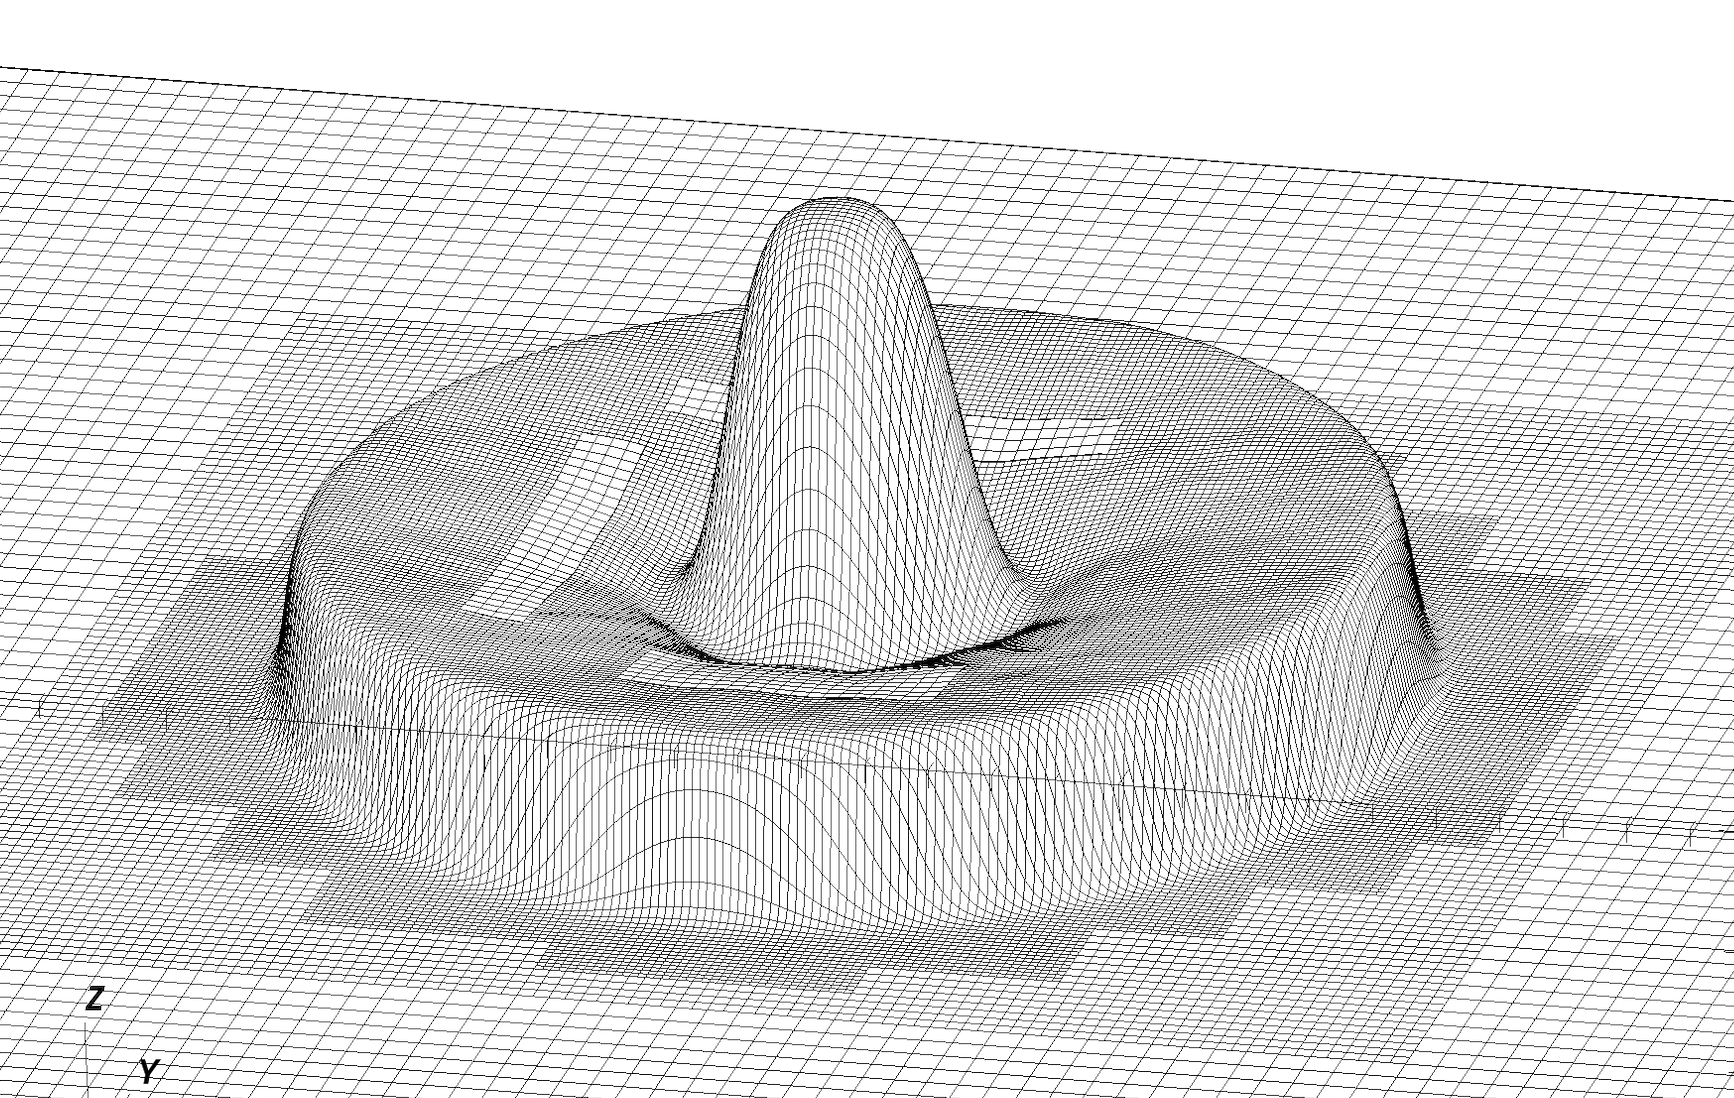
\includegraphics[width=\textwidth]{ShallowWater}
\end{frame}

\begin{frame}{Schardin Test Case}
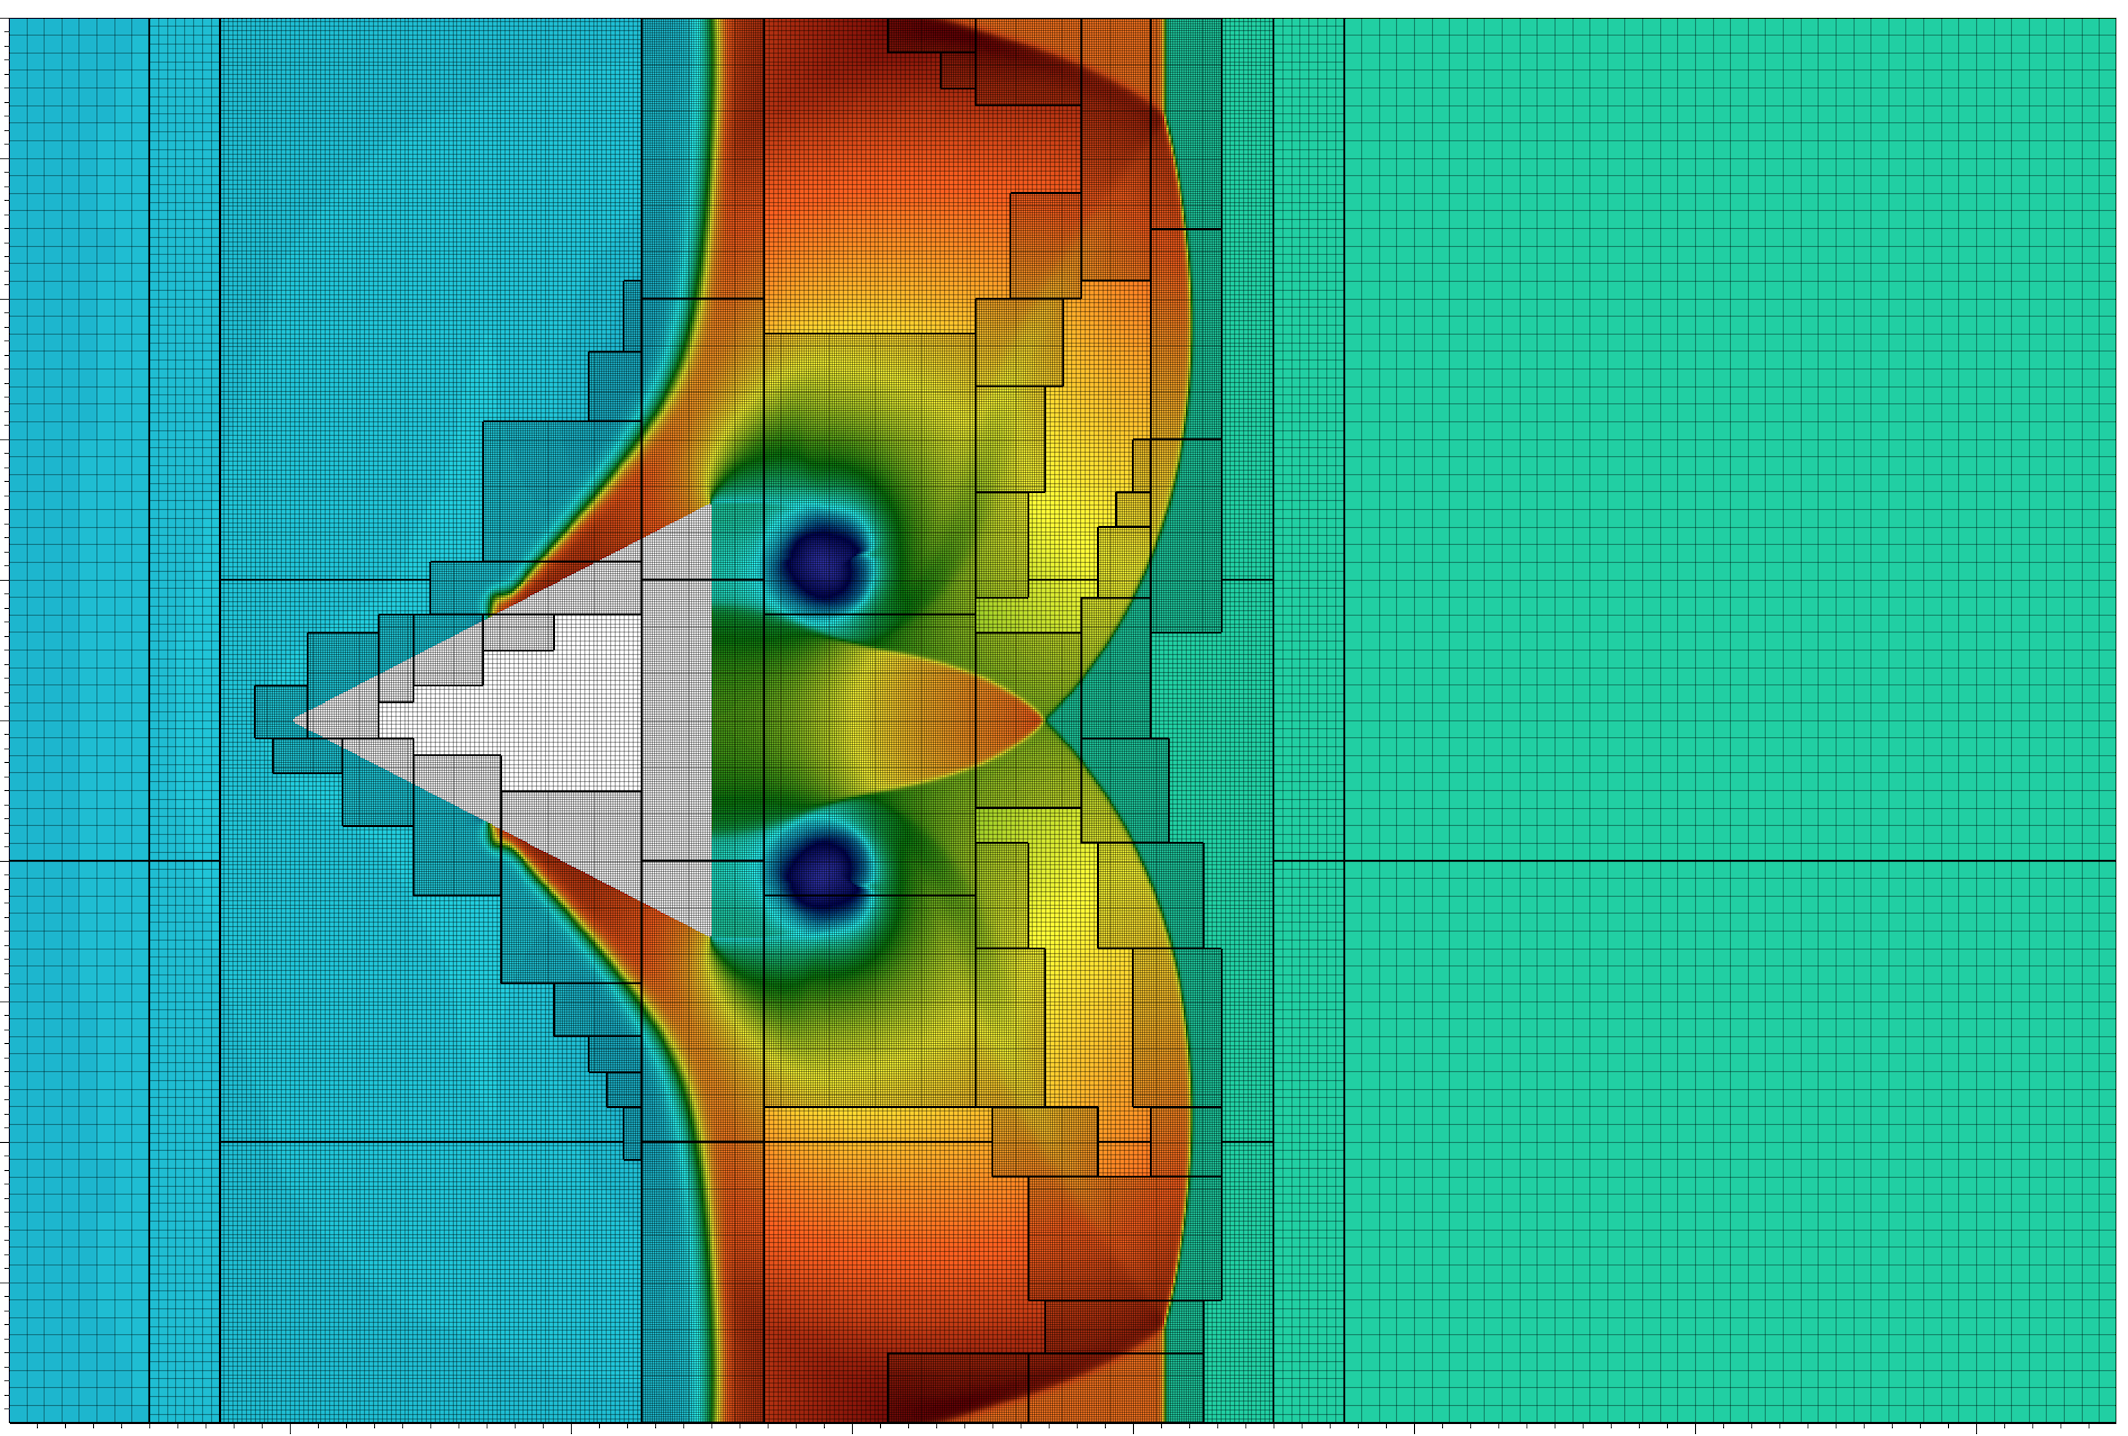
\includegraphics[width=\textwidth]{Schardin}
\end{frame}

\begin{frame}{Tube with Divider Geometry}
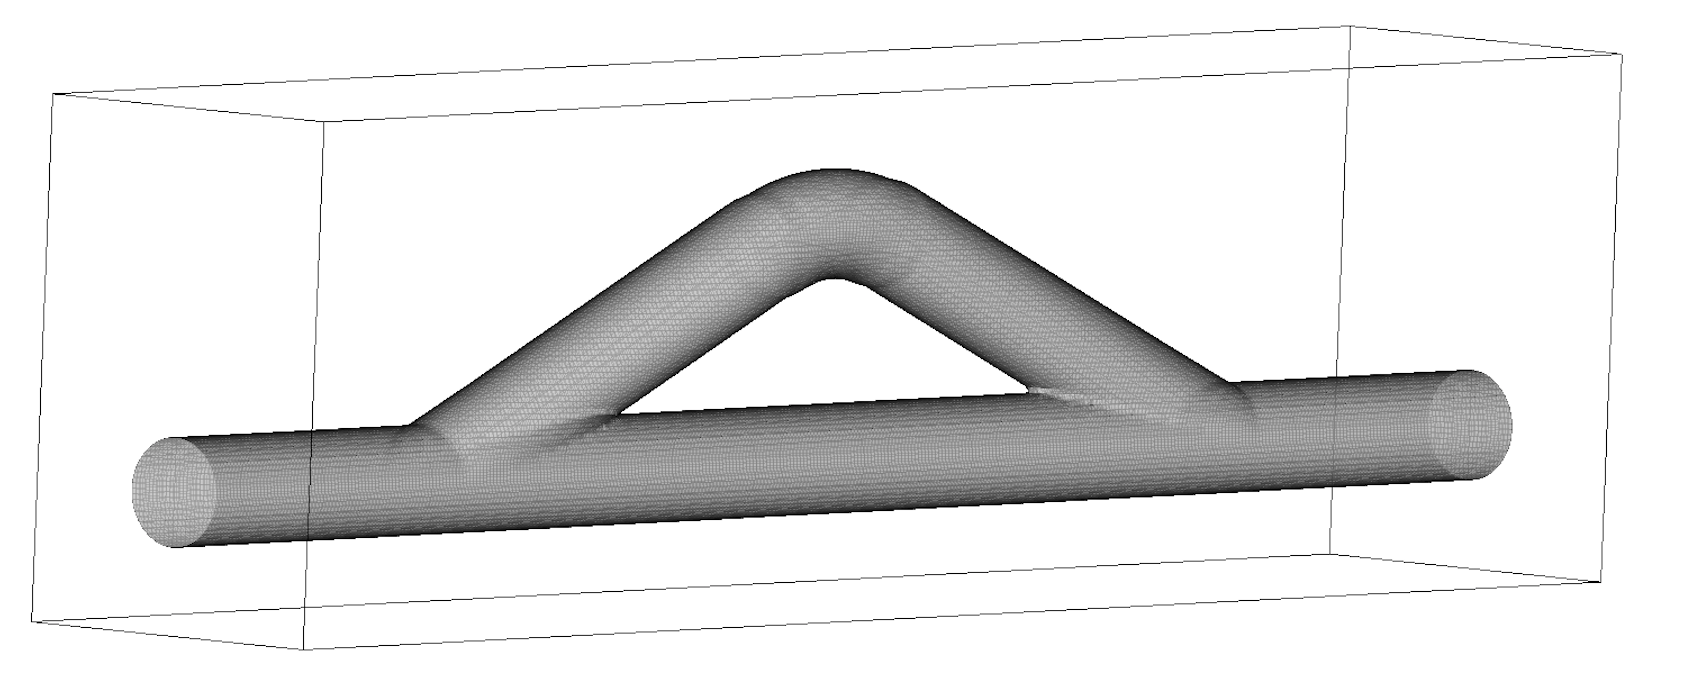
\includegraphics[width=\textwidth]{Divider} 
\end{frame}

\begin{frame}{Overview}
  \tableofcontents
\end{frame}

\section{Scope and Goals}
\begin{frame}{Scope and Goals of this library}
This library is driven by the following ideas
\begin{itemize}
	\item \textbf{not a final application code}
	\item provide building blocks for applications / concrete simulations
	\item building blocks are composable and efficient\\
	\begin{itemize} \item Make it easy to add specialized components \end{itemize}
	\item scale to moderately sized 3D problems on HLRN
	\item contiguously test mulitple target compilers on each commit
	\item nightly regression tests: reproduce simulation results to the past
	\item provide tools to postprocess simulation data

	\vspace{0.5cm}
	\item more control of the methods in my turbine simluations
\end{itemize}
\end{frame}


\begin{frame}{Common Tasks in a finite volume AMR simulation}
The library provides primitives for the following tasks

\vspace{0.4cm}
\begin{itemize}
	\item define an equation and its state variables
	\item store a distributed mesh with data
	\item initialize data
	\item setup boundary conditions
	\item tag cells for refinement
	\item perform finite volume methods
	\item output plot data
	\item create checkpoints to restart a simulation
	\item provide templates for a driver logic
	\item in-situ visualization (WIP)
\end{itemize}
\end{frame}

\begin{frame}{Current Library Size}
The library currently consists of approximately
\begin{itemize}
	\item $17.5$\,K lines of code
	\begin{itemize}
		\item STAFSEAsq: 60\,K lines of code
		\item LSC-AMR: 120\,K lines of code
	\end{itemize}
    \item 111 header files (.hpp) and 
    \item 40 source files (.cpp).
\end{itemize}

\vspace{1cm}
It features
\begin{itemize}
	\item AMR with either AMReX or SAMRAI backend
	\item very generic first and second order accurate finite volume methods based on given solutions to the riemann problem
	\item a dimensionally split method to handle embedded boundaries
\end{itemize}
\end{frame}
	
\section{Getting Started: Build and Install}

\begin{frame}{Overview}
\tableofcontents[currentsection]
\end{frame}

\begin{frame}{Getting Started}
There are multiple ways of getting started:

\vspace{0.3cm}
\begin{itemize}
	\item Manually install and configure all dependencies.\\
	      \emph{Use the package manager your OS, if possible}\\
          \emph{Best integration into native tools and IDEs}
          
    \vspace{0.3cm}
	\item Use our \textbf{conan} package recipes to get started with dependencies.
	      \emph{Requires you to have an installed MPI implementation}

    \vspace{0.3cm}
	\item Use one of our \textbf{docker} containers to compile your local code in a VM\\
	      \emph{Only recommended if your are not constantly developing} 
\end{itemize}
\end{frame}

\begin{frame}[fragile]{Conan Usage}
\texttt{conan} requires \texttt{Python} on your machine.
\\
Example:
\begin{lstlisting}[language=bash]
> pip3 install conan
> git clone https://git.imp.fu-berlin.de/ag-klima/FiniteVolumeSolver.git FiniteVolumeSolver/
> mkdir FiniteVolumeSolver/build && cd FiniteVolumeSolver/build
> conan remote add finite-volume https://api.bintray.com/conan/fub-agklein/finite-volume
> conan ../ install --build missing -o AMReX:dim=2 --env CXX=mpic++
> cmake ../ -DCMAKE_BUILD_TYPE="Release"
> make
\end{lstlisting}

Without conan you have to specify in the cmake configuration step all paths to dependencies manually
\begin{lstlisting}[language=bash]
> cmake ../ -Dfmt_DIR="{FMT_PREFIX}/lib/cmake/fmt"         \
            -DEigen3_DIR="{EIGEN3_PREFIX}/lib/cmake/Eigen" \
            -DBOOST_ROOT="{BOOST_PREFIX}"                  \
            -DAMReX_DIR="{AMREX_PREFIX}/lib/cmake/AMReX"   \
            -DCMAKE_BUILD_TYPE="Release"
\end{lstlisting}
\end{frame}

\begin{frame}[fragile]{Docker Usage}
You can use docker to compile the library with a preconfigured toolchain.
\\
Usage:
\begin{lstlisting}[language=bash]
> docker login git.imp.fu-berlin.de:5000
> docker run -v /Users/maikel/Development/FiniteVolumeSolver/:/FiniteVolumeSolver \
             -it git.imp.fu-berlin.de:5000/ag-klein/finitevolumesolver/amrex:2d_gcc7
> mkdir build && cd build
> conan install /FiniteVolumeSolver -o AMReX:dim=2
> cmake /FiniteVolumeSolver -DCMAKE_BUILD_TYPE="Release"
> make
\end{lstlisting}
\end{frame}

\section{Equations and its States and Views}
\begin{frame}{Overview}
\tableofcontents[currentsection]
\end{frame}

\begin{frame}{Define a new Equation}
To solve a hyperbolic equation with the current library you have to proceed in four steps

\vspace{0.3cm}
\begin{enumerate}
	\item declare conservative and complete state variables
	\item define a flux function $F$ as in $q_t + F(q)_x = 0$
	\item define how to obtain a complete state from a conservative one
	\begin{itemize} \item required if the states differ \end{itemize}
	\item define some solution to the riemann problem.
	\begin{itemize} \item alternatively define a flux method which does not use the solution to the riemann problem \end{itemize}
\end{enumerate}
\end{frame}

\begin{frame}[fragile]{States of an Equation}
The states of an \texttt{Equation} are denoted by \texttt{Conservative<Equation>} and \texttt{Complete<Equation>}.

\vspace{0.5cm}
1D Advection Equation:
\begin{lstlisting}
template <typename Mass> struct AdvectionVariables { Mass mass; };

struct Advection {
  using ConservativeShape = AdvectionVariables<Scalar>;
  using CompleteShape = AdvectionVariables<Scalar>;

  static constexpr int Rank() { return 1; }

  Conservative<Advection> Flux(Complete<Advection> q) const {
    return {.mass = velocity * q.mass};
  }

  double velocity{1.0};
};
\end{lstlisting}
\end{frame}

\begin{frame}[fragile]{1D Burgers Equation}
\begin{lstlisting}
template <typename U> struct BurgersVariables { U u; };

struct Burgers {
  using ConservativeShape = BurgersVariables<ScalarDepth>;
  using CompleteShape = BurgersVariables<ScalarDepth>;

  static constexpr int Rank() { return 1; }

  Conservative<Burgers> Flux(Complete<Burgers> q) const {
    return {.u = 0.5 * q.u * q.u};
  }
};
\end{lstlisting}
\end{frame}

\begin{frame}[fragile]{2D Shallow Water Equations}

\begin{lstlisting}
template <typename Height, typename Momentum> struct ShallowWaterVariables { 
  Height height;
  Momentum momentum;
};

struct ShallowWater2d {
  using ConservativeShape = ShallowWaterVariables<ScalarDepth, VectorDepth<2>>;
  using CompleteShape = ConservativeShape;

  static constexpr int Rank() { return 2; }

  Conservative<ShallowWater2d>
  Flux(const Complete<ShallowWater2d>& q, Direction dir) const {
    const int d = static_cast<int>(dir);
    const double velocity = q.momentum[d] / q.height;
    Conservative<ShallowWater2d> u{};
    u.height = q.momentum[d];
    u.momentum = velocity * q.momentum;
    u.momentum[d] += 0.5 * gravity_ * q.height * q.height;
    return u;
  }

  double gravity_;
};
\end{lstlisting}
\end{frame}

\begin{frame}[fragile]{Single Perfect Gas Euler Equations}
\begin{lstlisting}
template <typename Density, typename Momentum, typename Energy> 
struct PerfectGasCons { 
	Density density;
	Momentum momentum;
	Energy energy;
};

template <typename Density, typename Momentum, typename Energy, typename Pressure>
struct PerfectGasComplete : PerfectGasCons<Density, Momentum, Energy> {
	Pressure pressure;
};
\end{lstlisting}
\end{frame}

\begin{frame}[fragile]{Single Perfect Gas Euler Equations}
\begin{lstlisting}
template <int Dim>
struct PerfectGas {
  using ConservativeShape = PerfectGasCons<
    ScalarDepth,      // density
    VectorDepth<Dim>, // momentum
    ScalarDepth       // energy
  >;
  
  using CompleteShape = PerfectGasComplete<
    ScalarDepth,      // density
    VectorDepth<Dim>, // momentum
    ScalarDepth,      // energy
    ScalarDepth       // pressure
  >;
  static constexpr int Rank() { return Dim; }

  Conservative<PerfectGas>
  Flux(const Complete<PerfectGas>& q, Direction dir) const;
  
  Complete<PerfectGas> 
  CompleteFromCons(const Conservative<PerfectGas>& q) const;

  double gamma_{1.4};
};

extern template struct PerfectGas<1>;
extern template struct PerfectGas<2>;
extern template struct PerfectGas<3>;
\end{lstlisting}
\end{frame}

\begin{frame}[fragile]{Single Perfect Gas Euler Equations}
\begin{lstlisting}
template <int Dim>
Conservative<PerfectGas<Dim>> 
PerfectGas<Dim>::Flux(const Complete<PerfectGas<Dim>>& q, Direction dir) const {
  const int d = static_cast<int>(dir);
  const double velocity = q.momentum[d] / q.density;
  Conservative<PerfectGas<Dim>> flux{};
  flux.density = q.momentum[d];
  flux.momentum = velocity * q.momentum;
  flux.momentum[d] += q.pressure;
  flux.energy = velocity * (q.energy + q.pressure);
  return flux;
}

template <int Dim>
Complete<PerfectGas<Dim>> 
PerfectGas<Dim>::CompleteFromCons(const Conservative<PerfectGas<Dim>>& u) const {
  Complete<PerfectGas<Dim>> q{};
  AsCons(q) = u;
  const double e_kin = 0.5 * u.momentum.squaredNorm() / u.density;
  const double e_int = u.energy - e_kin;
  q.pressure = e_int * (gamma_ - 1.0);
  return q;
}

template struct PerfectGas<1>;
template struct PerfectGas<2>;
template struct PerfectGas<3>;
\end{lstlisting}
\end{frame}

\begin{frame}[fragile]{Ideal Gas Mixtures Euler Equations}
\begin{lstlisting}
template <int Dim>
struct IdealGasMix {
  using ConservativeShape = PerfectGasCons<
    ScalarDepth,                // density
    VectorDepth<Dim>,           // momentum
    ScalarDepth,                // energy
    VectorDepth<dynamic_extent> // species
  >;

  using CompleteShape = PerfectGasComplete<
    ScalarDepth,                // density
    VectorDepth<Dim>,           // momentum
    ScalarDepth,                // energy
    VectorDepth<dynamic_extent> // species
    ScalarDepth,                // pressure
    ScalarDepth,                // temperature
    ScalarDepth,                // heat_capacity_at_constant_pressure
    ScalarDepth                 // gamma
  >;
  static constexpr int Rank() { return Dim; }

  void Flux(Conservative<IdealGasMix>& flux, const Complete<IdealGasMix>& state,
            Direction dir) const;

  void CompleteFromCons(Complete<IdealGasMix>&,
                        const Conservative<IdealGasMix>&);

  FlameMasterReactor reactor_;
};
\end{lstlisting}
\end{frame}


\begin{frame}[fragile]{Solve the Riemann Problem}
\begin{lstlisting}
template <typename Equation> class ExactRiemannSolver;

template <> class ExactRiemannSolver<Advection> {
private:
  Advection equation_;

public:
  using Complete = ::fub::Complete<Advection>;

  explicit ExactRiemannSolver(Advection equation): equation_{equation} {}

  /// Returns either left or right, depending on the upwind velocity.
  void SolveRiemannProblem(Complete& sol, Complete left, Complete right) const;

  /// Returns the upwind velocity.
  std::array<double, 1> ComputeSignals(Complete left, Complete right) const;
};
\end{lstlisting}
\end{frame}

\begin{frame}[fragile]{Solve the Riemann Problem}
\begin{lstlisting}
void ExactRiemannSolver<Advection>::
SolveRiemannProblem(Complete& solution, Complete left, Complete right) const {
  if (equation_.velocity > 0) {
    solution = left;
  } else {
    solution = right;
  }
}

std::array<double, 1> ExactRiemannSolver<Advection2d>::
ComputeSignals(const Complete&, const Complete&) const {
  return {equation_.velocity};
}
\end{lstlisting}
\end{frame}

\begin{frame}[fragile]{State Transformations}
\begin{itemize}
	\item \texttt{Conservative<ShallowWater2d>}:
\begin{lstlisting}
Conservative<ShallowWater2d> = struct { 
  double                     height;
  Eigen::Array<double, 2, 1> momentum; 
};
\end{lstlisting}
  
  \item \texttt{ConservativeArray<ShallowWater2d, N>}:
\begin{lstlisting}
ConservativeArray<ShallowWater2d, N> = struct { 
  Eigen::Array<double, 1, N> height;
  Eigen::Array<double, 2, N> momentum; 
};
\end{lstlisting}

  \item \texttt{View<Conservative<ShallowWater2d> >}:
\begin{lstlisting}
View<Conservative<ShallowWater2d> > = struct { 
  PatchDataView<double, 2> height;
  PatchDataView<double, 3> momentum; 
};
\end{lstlisting}
\end{itemize}
\end{frame}


\begin{frame}[fragile]{State Transformations}
\begin{itemize}
\item \texttt{Complete to Conservative:}
\begin{lstlisting}
template <typename Eq> void f(Conservative<Eq>& u);

Complete<Eq> q = /* ... */;
f(q);                    // Error: can not deduce template parameter

Conservative<Eq>& u = q;
f(u);                    // Ok.
f(AsCons(q));            // Ok.
\end{lstlisting}
\item \texttt{Same for Views:}
\begin{lstlisting}
template <typename Eq> void f(const View<const Conservative<Eq> >& u);
View<Complete<ShallowWater> > view = /* ... */ 
f(AsConst(AsCons(view)));
\end{lstlisting}
\item \texttt{Iterate over all member variables in a generic context:}
\begin{lstlisting}
Complete<Eq> q, w;
// ...
ForEachVariable([](auto& qi, auto& wi) { /* ... */ }, AsCons(q), AsCons(w));
ForEachComponent([](double& qi, double wi) { /* ... */ }, AsCons(q), AsCons(w));
\end{lstlisting}
\end{itemize}
\end{frame}

\begin{frame}[fragile]{Use a View}
\begin{itemize}
\item iterate over all indices in range
\begin{lstlisting}
View<Complete<ShallowWater> > q = /* get view from AMReX or SAMRAI */
ForEachIndex(Box<0>(q), [&](std::ptrdiff_t i, std::ptrdiff_t j) {
  q.height(i, j) = 1.0;
  q.momentum(i, j, 0) = 1.0;
  q.momentum(i, j, 1) = 0.0;
}); 
\end{lstlisting}
\item iterate over a generic View
\begin{lstlisting}
View<const Complete<Eq> > states = /* get view from AMReX or SAMRAI */
View<Conservative<Eq> > fluxes = /* get view from AMReX or SAMRAI */
Complete left{equation};
Complete right{equation};
Conservative flux{equation};
ForEachIndex(Shrink(Box<0>(q), dir, {0, 1}), [&](auto... is) {
  const Index face{is...}
  const Index left = face;
  const Index right = Shift(left, dir, 1);
  Load(left, states, left);
  Load(right, states, left);
  ComputeNumericFluxes(flux, {left, right}, dir);
  Store(fluxes, flux, left);
}); 
\end{lstlisting}
\end{itemize}
\end{frame}

\section{Formulate Solver Primitives}
\begin{frame}{Overview}
\tableofcontents[currentsection]
\end{frame}

\begin{frame}{Flux Methods}
We provide some predefined flux methods which can be used in very generic contexts:

\begin{itemize}
	\item \texttt{GodunovMethod<Equation, RiemannSolver>}
	\item \texttt{HllMethod<Equation, SignalVelocities>}
	\item \texttt{MusclHancockMethod<Equation, BaseMethod, SlopeLimiter>}
\end{itemize}
\end{frame}

\begin{frame}[fragile]{First Order Godunov Method}
\begin{lstlisting}
template <typename Equation, typename RiemannSolver> class Godunov {
private:
  Equation equation_;
  RiemannSolver solver_;
  Complete<Equation> solution_;

public:
  explicit Godunov(const Equation& equation) : equation_{equation} {}

  void ComputeNumericFlux(Conservative<Equation>& numeric_flux,
                          span<const Complete<Equation>, 2> states,
                          Duration /* dt */, double /* dx */, Direction dir) {
    solver_.SolveRiemannProblem(solution_, states[0], states[1], dir);
    Flux(equation_, numeric_flux, solution_, dir);
  }

  double ComputeStableDt(span<const Complete<Equation>, 2> states, double dx,
                         Direction dir) {
    auto signals = riemann_solver_.ComputeSignals(states[0], states[1], dir);
    const double s_max = std::accumulate(
        signals.begin(), signals.end(), 0.0,
        [](double x, double y) { return std::max(x, std::abs(y)); });
    return dx / s_max;
  }
};
\end{lstlisting}
\end{frame}

\begin{frame}[fragile]{First Order Hll Method}
\begin{lstlisting}
template <typename Equation, typename SignalSpeeds> class Hll {
private:
  Equation equation_;
  SignalSpeeds signal_speeds_;
  Conservative<Equation> flux_left_{equation};
  Conservative<Equation> flux_right_{equation};

public:
  void ComputeNumericFlux(Conservative& numeric_flux,
                          span<const Complete, 2> states, Duration dt,
                          double dx, Direction dir);

  // ...
};
\end{lstlisting}
\end{frame}

\begin{frame}[fragile]{First Order Hll Method}
\begin{lstlisting}
template <typename Eq, typename SignalSpeeds>
void Hll<Eq, SignalSpeeds>::ComputeNumericFlux(
    Conservative<Eq>& numeric_flux, span<const Complete<Eq>, 2> states,
    Duration /* dt */, double /* dx */, Direction dir) {
  const Complete<Eq>& left = states[0];
  const Complete<Eq>& right = states[1];

  const auto signals = signal_speeds_(equation_, left, right, dir);

  Flux(equation_, flux_left_, left, dir);
  Flux(equation_, flux_right_, right, dir);

  const double sL = std::min(0.0, signals[0]);
  const double sR = std::max(0.0, signals[1]);
  const double sLsR = sL * sR;
  const double ds = sR - sL;
  FUB_ASSERT(ds > 0);

  ForEachComponent<Conservative>(
      [&](double& nf, double fL, double fR, double qL, double qR) {
        nf = (sR * fL - sL * fR + sLsR * (qR - qL)) / ds;
      },
      numeric_flux, flux_left, flux_right, states[0], states[1]);
}
\end{lstlisting}
\end{frame}


\begin{frame}[fragile]{Second Order Muscl Hancock Method}
\begin{lstlisting}
template <typename EquationT,
          typename BaseMethod =
              GodunovMethod<EquationT, ExactRiemannSolver<EquationT>>,
          typename SlopeLimiter = MinMod>
struct MusclHancock {
private:
  // These member variables control the behaviour of this method
  Equation equation_;
  BaseMethod flux_method_;
  SlopeLimiter slope_limiter_;

  // These member variables are used as an intermediate computation storage
  // and need to be allocated at construction time.
  std::array<Complete, 2> rec_{Complete{equation_}, Complete{equation_}};
  Conservative slope_{equation_};     //< Storage for the limited slopes
  Conservative flux_left_{equation_}; //< Storage for an intermediate left flux
  Conservative flux_right_{equation_}; //< Storage for an right flux
  Complete q_left_{equation_};  //< Storage for an intermediate left state
  Complete q_right_{equation_}; //< Storage for an intermediate right state

public:
  MusclHancock(const Equation& eq, const BaseMethod& method, 
               const SlopeLimiter& slopes = SlopeLimiter())
      : equation_{eq}, flux_method_{method}, slope_limiter_{sloeps} {}

  static constexpr int GetStencilWidth() noexcept { return 2; }

  void ComputeNumericFlux(Conservative& flux, span<const Complete, 4> stencil,
                          Duration dt, double dx, Direction dir);
};
\end{lstlisting}
\end{frame}

\begin{frame}[fragile]{Implementation: Part I}
\begin{lstlisting}
void ComputeNumericFlux(Conservative& flux, span<const Complete, 4> stencil,
                        Duration dt, double dx, Direction dir) {
  const double lambda_half = 0.5 * dt.count() / dx;

  // Compute Left Reconstructed Complete State

  slope_limiter_.ComputeLimitedSlope(slope_, stencil.template first<3>());

  ForEachComponent<Conservative>(
      [](double& qL, double& qR, double state, double slope) {
        qL = state - 0.5 * slope;
        qR = state + 0.5 * slope;
      },
      q_left_, q_right_, stencil[1], slope_);

  CompleteFromCons(equation_, q_left_, q_left_);
  CompleteFromCons(equation_, q_right_, q_right_);

  Flux(equation_, flux_left_, q_left_, dir);
  Flux(equation_, flux_right_, q_right_, dir);

  ForEachComponent<Conservative>(
      [&lambda_half](double& rec, double qR, double fL, double fR) {
        rec = qR + lambda_half * (fL - fR);
      },
      rec_[0], q_right_, flux_left_, flux_right_);

  CompleteFromCons(equation_, rec_[0], rec_[0]);
\end{lstlisting}
\end{frame}

\begin{frame}[fragile]{Implementation: Part II}
\begin{lstlisting}
  // Compute Right Reconstructed Complete State

  slope_limiter_.ComputeLimitedSlope(slope_, stencil.template last<3>());

  ForEachComponent<Conservative>(
      [](double& qL, double& qR, double state, double slope) {
        qL = state - 0.5 * slope;
        qR = state + 0.5 * slope;
      },
      q_left_, q_right_, stencil[2], slope_);

  CompleteFromCons(equation_, q_left_, q_left_);
  CompleteFromCons(equation_, q_right_, q_right_);

  Flux(equation_, flux_left_, q_left_, dir);
  Flux(equation_, flux_right_, q_right_, dir);

  ForEachComponent<Conservative>(
      [&lambda_half](double& rec, double qL, double fL, double fR) {
        rec = qL + lambda_half * (fL - fR);
      },
      rec_[1], q_left_, flux_left_, flux_right_);

  CompleteFromCons(equation_, rec_[1], rec_[1]);

  // Invoke Lower Order Flux Method

  flux_method_.ComputeNumericFlux(flux, span{rec_}, dt, dx, dir);
}
\end{lstlisting}
\end{frame}

\section{Initialize Data}
\begin{frame}{Overview}
\tableofcontents[currentsection]
\end{frame}

\begin{frame}[fragile]{The Dam Break Problem}
\begin{lstlisting}
struct RiemannProblem {
  PerfectGas<1> equation_;
  void
  InitializeData(const View<Complete<PerfectGas<1>>>& states,
                 const amrex::PatchHierarchy& hierarchy,
                 amrex::PatchHandle patch) const {
    const ::amrex::Geometry& geom = hierarchy.GetGeometry(patch.level);
    const ::amrex::Box& box = patch.iterator->tilebox();
    CartesianCoordinates x =
        amrex::GetCartesianCoordinates(geom, box);
    Complete<PerfectGas<1>> complete{equation_};
    ForEachIndex(Box<0>(states), [&](auto... is) {
      Conservative<PerfectGas<1>> state{equation_};
      if (x(is...)[0] < 0.0) {
        state.energy = 8.0 * equation_.gamma_minus_1_inv;
      } else {
        state.energy = 1.0 * equation_.gamma_minus_1_inv;
      }
      state.density = 1.0;
      state.momentum.fill(0);
      CompleteFromCons(equation_, complete, state);
      Store(states, complete, {is...});
    });
  }
};
\end{lstlisting}
\end{frame}

\section{Setup Boundary Conditions}
\begin{frame}{Overview}
\tableofcontents[currentsection]
\end{frame}

\begin{frame}
There are currently some pre-defined boundary conditions which can be used
\vspace{0.4cm}
\begin{itemize}
	\item \texttt{BoundarySet}
	\item \texttt{TransmissiveBoundary}
	\item \texttt{ReflectiveBoundary}
	\item \texttt{IsentropicExpansionBoundary}
	\item \texttt{MassflowBoundary}
	\item \texttt{CoupledBoundary}
	\item \texttt{PeriodicBoundary} (not really a class)
\end{itemize}
\end{frame}

\section{Run a Simulation}
\begin{frame}{Overview}
\tableofcontents[currentsection]
\end{frame}

\begin{frame}[fragile]
To run a simulation you have to proceed in the following steps
\vspace{0.4cm}
\begin{enumerate}
	\item Construct a \texttt{std::shared\_ptr<GriddingAlgorithm>} and initialize the \texttt{PatchHierarchy}.
\begin{lstlisting}
struct GriddingAlgorithm {
  PatchHierarchy hierarchy_;
  BoundaryCondition boundary_condition_;
  InitialCondition intial_condition_;
  TaggingStrategy tagging_;
};
\end{lstlisting}
	\item Construct a solver object using a \texttt{FluxMethod} and \texttt{TimeIntegrator}.
	\item Setup your output and call \texttt{RunSimulation}.
\end{enumerate}
\end{frame}

\end{document}